\chapter{Implementierung} % (fold)
\label{sec:implementierung}
Nachfolgend soll die Implementierung der verschiedenen APIs, sowie die Grundprinzipien während der Implementierung, beschrieben werden. Der Source Code der Implementierung ist unter MIT Lizenz auf GitHub veröffentlicht. \citep{me}
\section{Grundprinzipien während der Implementierung} % (fold)
\label{sec:prinzipien}
Im Rahmen der Implementierung dieser Anwendung wurden verschiedene Grundprinzipien beachtet, die sowohl die Qualität als auch die Erweiterbarkeit der Anwendungen  sicherstellen. Die Wahl der verwendeten Technologien sowie die Anwendung bewährter Praktiken standen dabei im Vordergrund. Als Basis für die Entwicklung wurde Java JDK 17.0.10 Corretto gewählt, da diese als Long-Term-Support (LTS-Version) eine stabile und sichere Grundlage für die Entwicklung darstellt. Amazon Corretto bietet eine optimierte JVM, wodurch alle Softwarebestandteile auf jeder Plattform mit einer zertifizierten JAVA Virtual Machine lauffähig sind. Ergänzt wurde das JDK durch Spring Boot Version 3.3.4, eine weit verbreitete Plattform für die Entwicklung von Webanwendungen und Microservices. Spring Boot ermöglicht eine schnelle und einfache Konfiguration von Anwendungen und vereinfacht den Entwicklungsprozess durch das Automatisieren von häufig auftretenden Aufgaben, wie etwa der Konfiguration von Servern und Datenbankverbindungen.
\noindent
Ein zentrales Konzept während der Implementierung war die Verwendung von Dependency Injection (DI). Diese Technik sorgt dafür, dass die Abhängigkeiten zwischen den einzelnen Komponenten der Anwendung nicht hartkodiert sind, sondern zur Laufzeit durch den DI-Container von Spring injiziert werden. DI fördert die Entkopplung von Komponenten, was zu einer besseren Testbarkeit, Flexibilität und Wartbarkeit des Codes führt. Da der Code durch DI in unabhängige, gut getestete Module unterteilt wird, lässt er sich leicht erweitern und an geänderte Anforderungen anpassen. Zudem trägt DI zur Verbesserung der Lesbarkeit des Codes bei, da Abhängigkeiten nicht explizit an anderen Stellen erstellt werden müssen.
\noindent
Die Implementierung der Anwendung erfolgte unter der Berücksichtigung von Best Practices, die die Qualität des Codes sicherstellen und eine effiziente, langfristige Wartung ermöglichen. Ein wesentlicher Aspekt war hierbei die Modularität der Lösung. Die Anwendung wurde so strukturiert, dass jede Komponente eine klare, abgegrenzte Verantwortung übernimmt. Dies sorgt nicht nur für eine bessere Nachvollziehbarkeit des Codes, sondern erleichtert auch das Testen und die Erweiterung von Funktionalitäten. Bestehende Komponenten können so problemlos durch neue ersetzt oder erweitert werden, ohne die gesamte Anwendung zu beeinträchtigen.




% section prinzipien (end)

\section{Post REST} % (fold)
\label{sec:postrest}
In dieser Arbeit steht "PostREST" für die PostgreSQL REST-API, die eine Schnittstelle für den Zugriff auf eine PostgreSQL-Datenbank über HTTP-Anfragen bietet. Diese API implementiert eine Reihe von Endpunkten, die in Abschnitt 5.2.1 der Arbeit definiert sind. Diese Endpunkte sind dafür verantwortlich, bestimmte Anfragen zu bearbeiten und entsprechende Antworten zurückzugeben.
\noindent
Die zentrale Komponente, die dafür sorgt, dass die Endpunkte korrekt verarbeitet werden, ist die Controller-Klasse(vgl Abb. 6.1). In dieser Klasse sind die Endpunkte integriert, wobei jeder Endpunkt mit seinen spezifischen Pfadvariablen und den Rückgabewerten versehen ist. Die Controller-Klasse übernimmt die Aufgabe, die richtigen Methoden auszuführen, wenn eine Anfrage an einen bestimmten Endpunkt gestellt wird.
\noindent
Der PostrestController ist die konkrete Implementierung des Controllers, der die Geschäftslogik verarbeitet. Er ruft den DBService auf, welcher das Interface IDBService implementiert. Das Interface definiert die Methoden, die notwendig sind, um Daten aus den zugrunde liegenden Datenbanken abzurufen. Diese Methoden kapseln die Logik für den Datenbankzugriff und sind so gestaltet, dass sie von der Controller-Klasse verwendet werden können, um die richtigen Informationen zu erhalten.
\noindent
Die Kommunikation zwischen den verschiedenen Schichten der Anwendung erfolgt durch Dependency Injection. Das bedeutet, dass die verschiedenen Komponenten nicht direkt in der Controller-Klasse erzeugt werden, sondern von außen in die Klasse injiziert werden. In diesem Fall werden die Repositorys der verschiedenen Entitäten in die Controller-Klasse injiziert. Diese Repositorys sind verantwortlich für den direkten Datenbankzugriff und beinhalten die notwendigen Methoden und SQL-Abfragen, die zum Abrufen und Verwalten der Daten in der Datenbank erforderlich sind.
\noindent
Nachdem die Daten erfolgreich aus der Datenbank abgefragt wurden, werden sie durch die Hierarchie der Anwendung weitergegeben. Der PostrestController sorgt dafür, dass die abgerufenen Daten in das gewünschte Format für die API-Antwort umgewandelt werden. Dies ist in diesem Fall das JSON-Format, dass dann dem Nutzer der API als Antwort übermittelt wird. Diese Antwort enthält die angeforderten Informationen, die der Nutzer über die API abgefragt hat.
\begin{figure}[H]
	\centering
	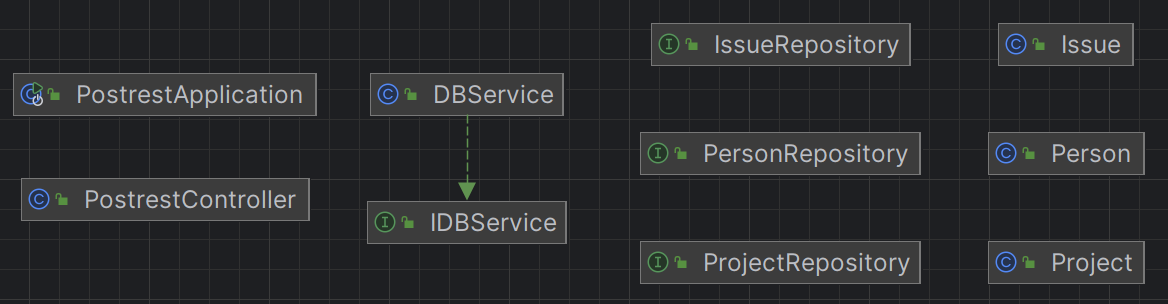
\includegraphics[scale=0.5]{Illustrations/postrest.png}
	\caption{Java Klassen PostREST}
\end{figure}
% section postrest (end)

\section{Post Graph} % (fold)
\label{sec:postgraph}
Hierbei handelt es sich um eine GraphQL-API, die mit einer PostgreSQL-Datenbank verbunden ist. Das Schema, das die Arbeitsweise der API beschreibt, wird – wie bei GraphQL üblich – in der Datei schema.graphqls definiert. In dieser Datei sind die verschiedenen Datentypen sowie die möglichen Queries und Mutationen beschrieben, die zur Abfrage und Bearbeitung der Daten verwendet werden können. 
\noindent
In den folgenden Abbildungen sind Beispiele für einen Typ, verschiedene Queries und eine Mutation dargestellt, wie sie in der schema.graphqls-Datei definiert sind:
\begin{figure}[H]
\begin{center}
\begin{BVerbatim}
type Issue{
    iid : ID!
    title : String
    createdAt : String
    state : String
    stateReason : String
}
\end{BVerbatim}
\end{center}
\caption{Type aus der Schema.graphqls}
\end{figure}
\begin{figure}[H]
\begin{center}
\begin{BVerbatim}
type Query{
    persons: [Person]
    person(id:ID!): Person
    projects: [Project]
    project(id:ID!) : Project
    issues : [Issue]
    issue(id: String): Issue
}
\end{BVerbatim}
\end{center}
\caption{Queries aus der Schema.graphqls}
\end{figure}
\begin{figure}[H]
\begin{center}
\begin{BVerbatim}

type Mutation {
    createIssue(input: IssueInput): Issue
}
\end{BVerbatim}
\end{center}
\caption{Mutation aus der Schema.graphqls}
\end{figure}
\newpage
\noindent
Die zentrale Komponente für die Verarbeitung von Anfragen ist die Java-Klasse Query(vgl. Abb. 6.5). In dieser Klasse werden Methoden implementiert, die die Bearbeitung der Anfragen gemäß den Strukturen in der schema.graphqls-Datei ermöglichen. Diese Methoden greifen auf die Repositories der Modelklassen zu, um Datenbankoperationen durchzuführen. Die Repositories enthalten die erforderlichen Methoden und Logiken, um Daten in der PostgreSQL-Datenbank zu lesen oder zu ändern.
\noindent
Ein hervorstechendes Merkmal von GraphQL ist der Einsatz von Resolvern. Diese kommen zum Einsatz, um Felder zu verarbeiten, die auf Daten aus anderen Quellen oder Datenbanken basieren. Resolver stellen sicher, dass die relevanten Daten korrekt abgerufen und in der gewünschten Struktur zurückgegeben werden.
\noindent
Die Repositories werden in die benötigten Klassen injiziert, sodass sie nicht direkt innerhalb der Anwendung erstellt werden müssen.
\noindent
Nach erfolgreicher Bearbeitung einer Anfrage liefert die GraphQL-API die Daten im vorgegebenen GraphQL-Format an den Nutzer zurück. Dies gewährleistet eine flexible und leistungsfähige Schnittstelle zur Abfrage und Manipulation der Daten in der zugrunde liegenden PostgreSQL-Datenbank.
\begin{figure}[H]
	\centering
	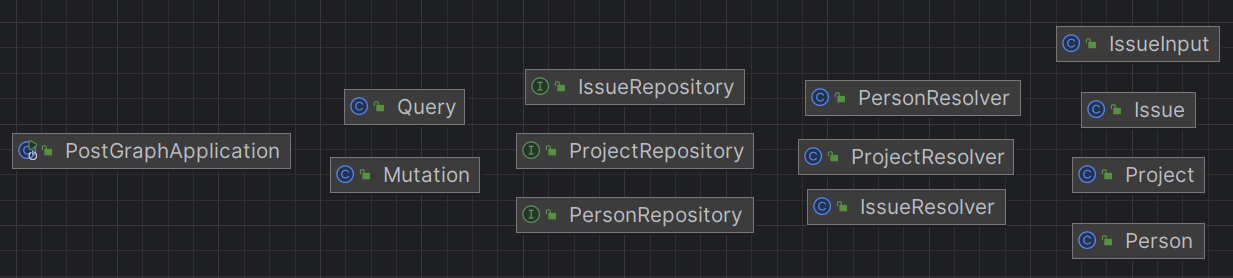
\includegraphics[scale=0.5]{Illustrations/postgraph.png}
	\caption{Java Klassen PostGraph}
\end{figure}
% section postgraph (end)

\section{Neo4REST} % (fold)
\label{sec:neo4rest}
Neo4REST ist eine REST-API, die den Zugriff auf eine Neo4j-Datenbank ermöglicht. Analog zur Struktur von PostREST bietet Neo4REST eine Reihe von Endpunkten, die zur Bearbeitung spezifischer Anfragen und zur Rückgabe der entsprechenden Antworten dienen. Die Details dieser Endpunkte sind in Abschnitt 5.2.2 definiert.
\noindent 
Die Verarbeitung der Endpunkte wird durch die zentrale Controller-Klasse sichergestellt (vgl. Abb. 6.7). Wie bei PostREST sind hier die spezifischen Pfadvariablen, Parameter und Rückgabewerte der Endpunkte definiert. Die Controller-Klasse sorgt dafür, dass die passenden Methoden aufgerufen werden, sobald eine Anfrage an einen der Endpunkte gestellt wird.
\noindent 
Der Neo4RestController übernimmt dabei die Geschäftslogik und delegiert datenbankbezogene Aufgaben an den DBService, der das Interface IDBService implementiert. Dieses Interface definiert die für den Zugriff auf die Neo4j-Datenbank erforderlichen Methoden. Die Umsetzung der konkreten Abfragen erfolgt über Repositories, die für die Durchführung der Cypher-Abfragen zuständig sind. Diese Repositorys abstrahieren den Datenbankzugriff und bieten wiederverwendbare Methoden, um auf die in Neo4j gespeicherten Daten zuzugreifen oder sie zu ändern.
\noindent 
Die in der Datenbank abgefragten Informationen werden, wie auch bei PostREST, durch die Schichten der Anwendung weitergeleitet und im Controller in das JSON-Format umgewandelt, bevor sie als API-Antwort zurückgegeben werden. So stellt Neo4REST sicher, dass der Nutzer die angeforderten Informationen oder den Status einer Operation im passenden Format erhält.
\begin{figure}[H]
	\centering
	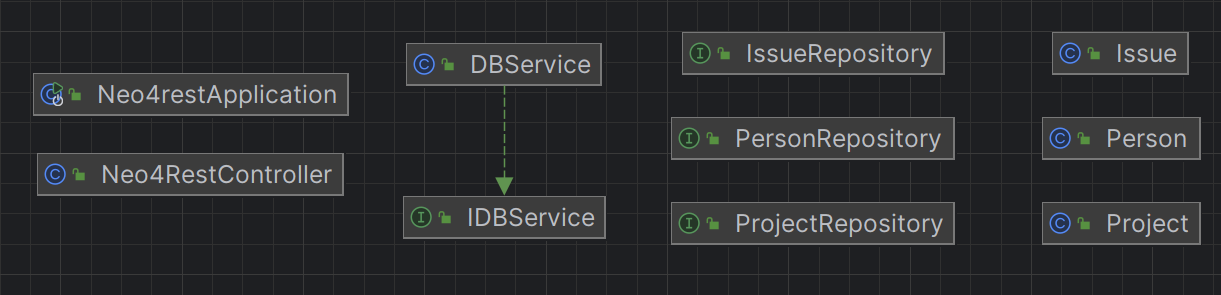
\includegraphics[scale=0.5]{Illustrations/neo4rest.png}
	\caption{Java Klassen Neo4REST}
\end{figure}
% section neo4rest (end)

\section{Neo4Graph} % (fold)
\label{sec:neo4graph}
Die Neo4Graph-API ist eine GraphQL-API, die mit einer Neo4j-Datenbank verbunden ist. Das Schema, das bereits in der PostGraph-API beschrieben wurde, wird auch in Neo4Graph auf ähnliche Weise implementiert. Wie bei PostGraph kommen auch hier Cypher-Abfragen zum Einsatz, um mit der Neo4j-Datenbank zu interagieren. Die Methoden nutzen die Neo4j-Clientbibliothek, um Knoten und Kanten effizient zu durchsuchen und Datenbankoperationen durchzuführen.
\noindent
Ein weiteres gemeinsames Merkmal beider APIs ist der Einsatz von Resolvern. In Neo4Graph werden diese ebenfalls verwendet, um Felder zu bearbeiten, die auf Beziehungen oder aggregierten Daten im Graphen basieren. Resolver sorgen dafür, dass die benötigten Daten korrekt abgerufen und in der gewünschten Struktur zurückgegeben werden.
\noindent
Nach der Bearbeitung einer Anfrage liefert die GraphQL-API die Daten im standardisierten GraphQL-Format an den Nutzer, was eine konsistente und leistungsfähige Schnittstelle zur Abfrage und Bearbeitung der Daten in der Neo4j-Datenbank sicherstellt

\begin{figure}[H]
	\centering
	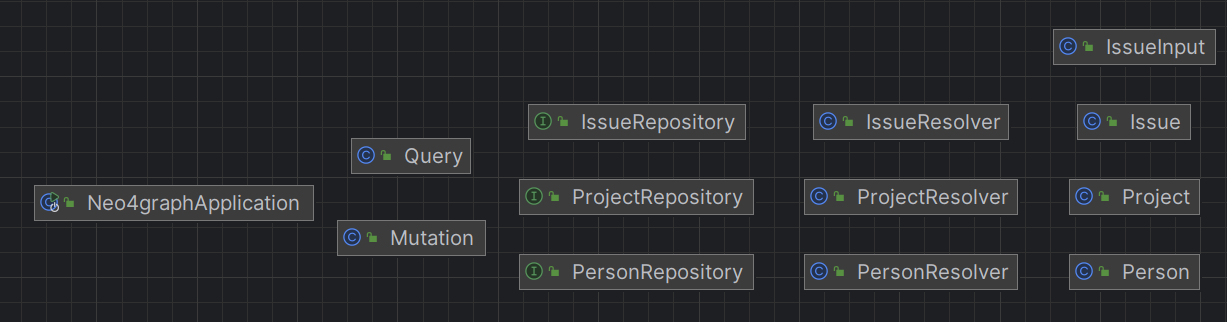
\includegraphics[scale=0.5]{Illustrations/neo4graph.png}
	\caption{Java Klassen Neo4Graph}
\end{figure}
% section neo4graph (end)
\section{API-Response Test} % (fold)
\label{sec:test}
Um API-Anfragen von einem entfernten System aus zu ermöglichen, wurde hierfür eine Anwendung entwickelt. Diese enthält für jeden Endpunkt eine Methode(vgl. Abb. 6.8), die jeweils 100 Abfragen in einer Schleife ausführt. Falls für eine Abfrage eine ID erforderlich ist, wird diese mithilfe der Klasse Random aus java.util.Random generiert. Die Abfragen für den parametrisierten Endpunkt werden mit den Joins von 0 bis 3 und den Ergebnistupeln 1, 100, 1000, 10.000 und 100.000 durchgeführt. Die Abfragezeit wird ermittelt, indem die aktuelle Systemzeit in Millisekunden unmittelbar vor der Ausführung der Abfrage erfasst und von der Zeit nach Abschluss der Abfrage abgezogen wird.
\begin{figure}[H]
	\centering
	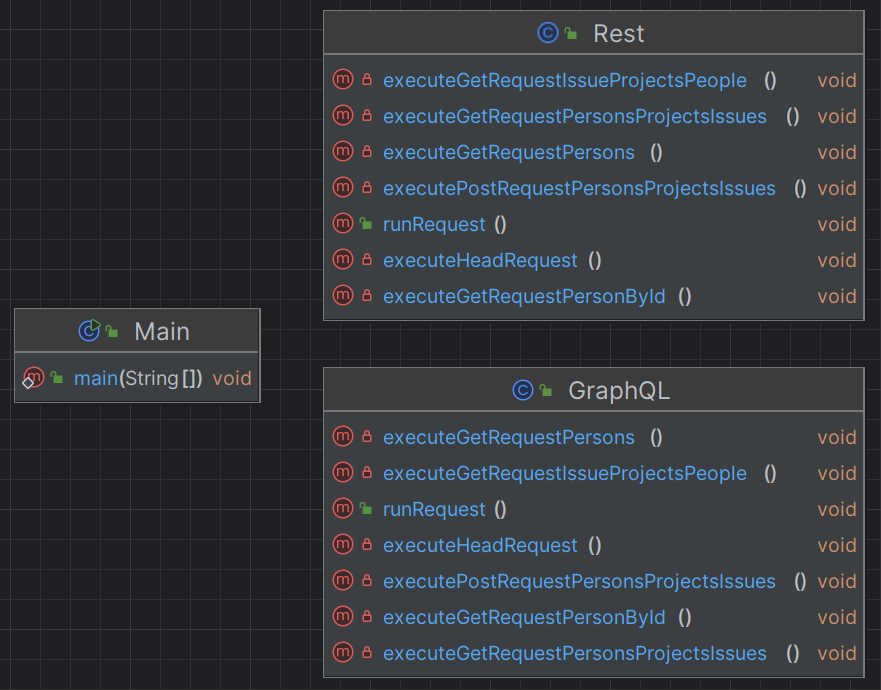
\includegraphics[scale=0.5]{Illustrations/apiresponsetest.png}
	\caption{Java Klassen Neo4Graph}
\end{figure}
% section test (end)
% chapter implementierung (end)